\chapter{Probar tu estación}\label{cap:pruebas}

Este capítulo tiene dos mitades: lo que ya se ha probado de la librería (y qué no), y cómo probar tú tu estación, incluida la primera vez en la maqueta real.

\section{Qué se ha probado ya}
\subsection{El simulador del grupo}
Para no depender de la maqueta, se ha construido un simulador que ejecuta \textbf{el código SCL de la librería tal cual sale de TIA Portal} y lo conecta a un modelo de la estación: una cinta con un palet, el stopper, y un lector RFID \emph{con el comportamiento del lector real} (sin eco de la orden, dato válido solo cuando «listo» baja y vuelve a subir, bloque de 28 bytes). La aplicación de cada estación se modela con el contrato de la librería.

Con él se hicieron \textbf{48 comprobaciones}, todas correctas con la versión \vlib. La lista completa está al final del capítulo; en resumen:
\begin{itemize}
\item Las cuatro estaciones (Cámara, BackCover, Press y Out), con sus máscaras: el palet completa el ciclo, la aplicación solo ve los bytes de su máscara de lectura, el tag queda como se espera y los bytes ajenos no cambian.
\item La plantilla de aplicación, sin tocar, completa un ciclo con la librería.
\item Un fallo del RFID lleva a la etapa 6, no arranca la aplicación, no escribe nada, y tras el rearme el palet sale.
\item Una emergencia durante la aplicación detiene la cinta y el stopper, no escribe nada en el tag, y tras soltar la seta y rearmar se vuelve a la normalidad.
\item Los tres ejemplos de aplicación (Press, BackCover y Cámara), con modelos sencillos de su hardware.
\end{itemize}

\subsection{Lo que encontraron las pruebas}
Las pruebas sirvieron: \textbf{encontraron un error en la versión 1.0.0 de la librería}. En \cod{Est\_FB\_Estacion}, la condición que apaga la cinta estaba escrita al revés (\cod{IF NOT Inhibir\_cinta THEN Cinta\_dch := FALSE}), de modo que la cinta se apagaba siempre que la aplicación \emph{no} la inhibía, es decir, siempre. Con esa versión, 17 de las 30 comprobaciones de la librería fallaban: la cinta nunca arrancaba. Está corregido en la versión \vlib\ (\cod{IF Inhibir\_cinta THEN}). Si tu archivo es el \texttt{v1.0.0}, pide el \texttt{v\vlib}.

\begin{peligro}
Usa siempre la versión \vlib\ o posterior. La 1.0.0 no mueve la cinta.
\end{peligro}

\subsection{Cómo se ve un ciclo}
Las dos figuras siguientes son del simulador. En la primera, un palet por la estación Cámara (la figura~\ref{fig:crono} del capítulo~\ref{cap:vision}); en la segunda, por la estación Out, que al final escribe el bloque a cero. Las etapas (arriba) cambian siempre en el mismo orden.

\begin{figure}[ht]
\centering
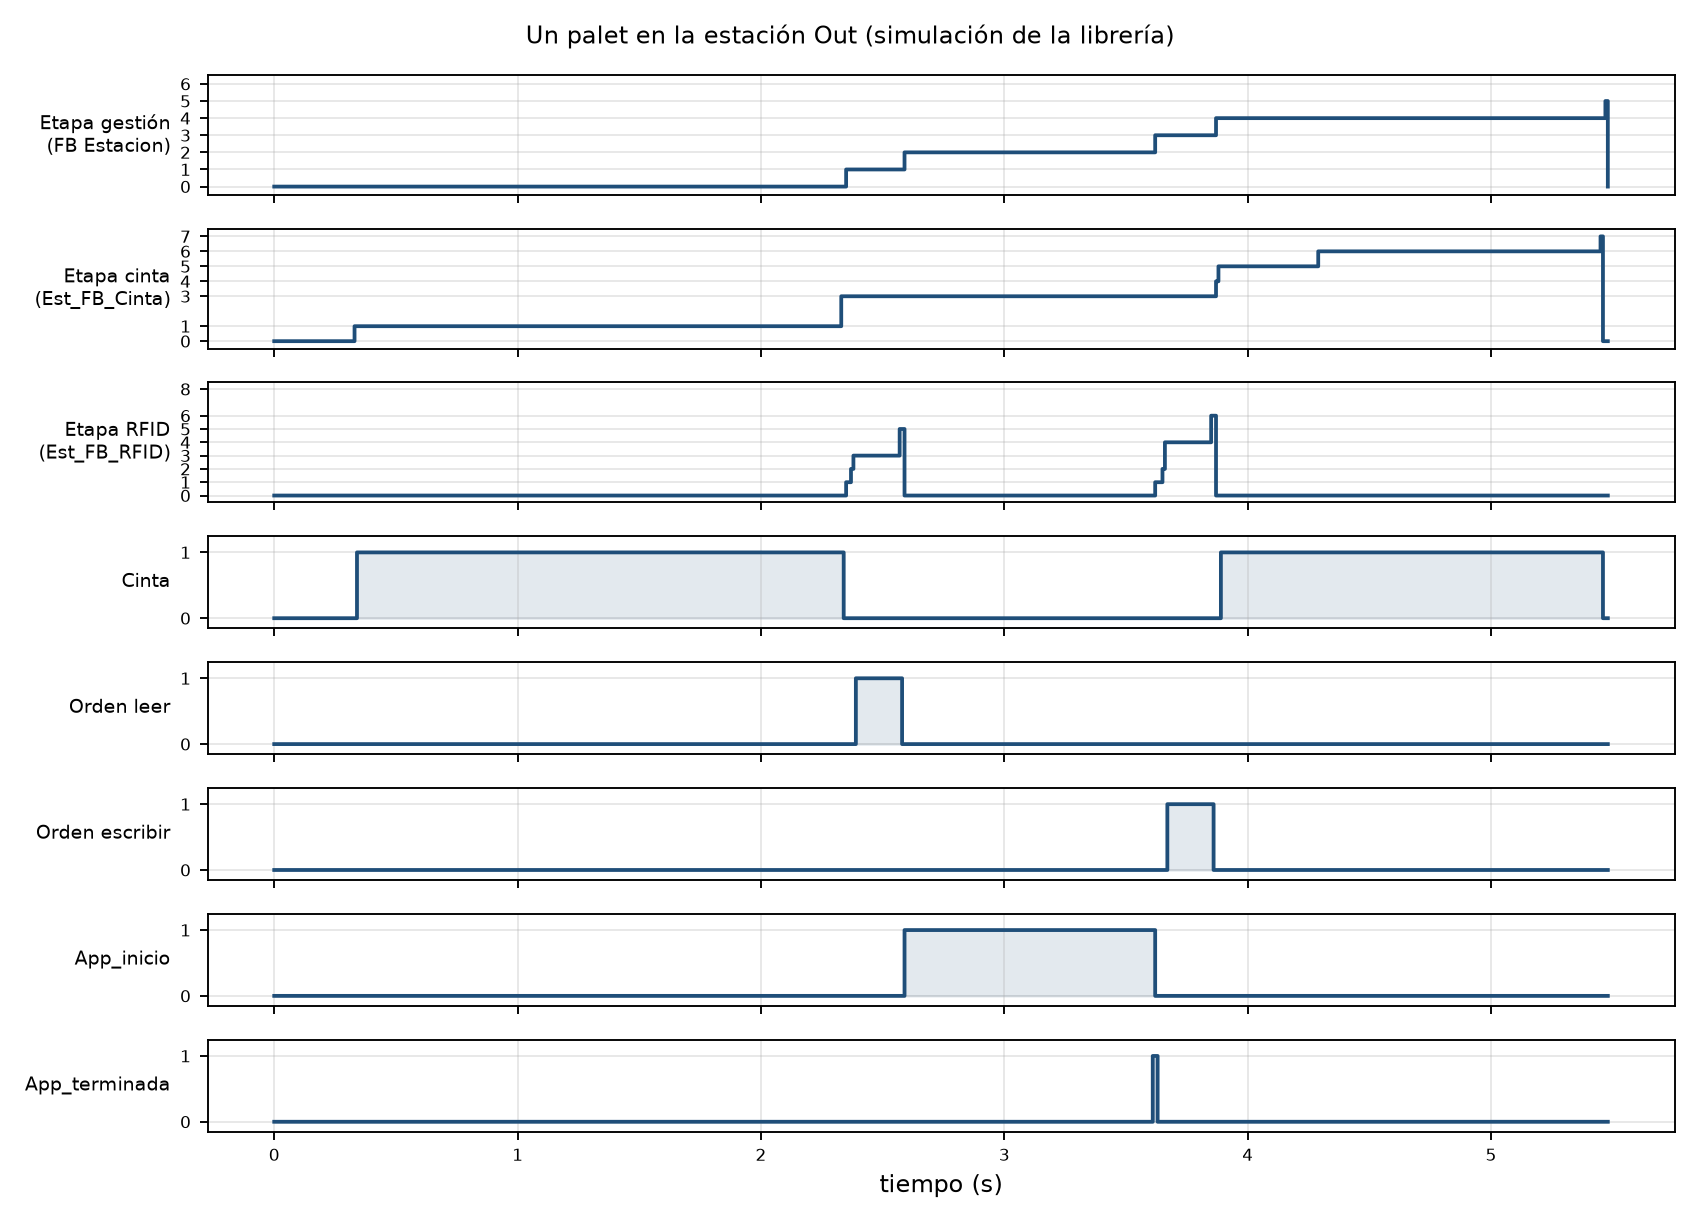
\includegraphics[width=\textwidth]{figuras/crono_ciclo_out.png}
\caption{Un palet en la estación Out (simulación).}
\end{figure}

\subsection{Qué \emph{no} cubre el simulador}
\begin{itemize}
\item \textbf{El hardware real}: tiempos de IO-Link, ruido, polaridad de cada sensor, señales que no están conectadas.
\item \textbf{El PROFINET}, la HMI y las comunicaciones con otros PLC (cámara, Festo).
\item \textbf{Varios palets pegados} en la cinta (en la estación Out se probó con el simulador de CIROS, no con este).
\item \textbf{Tu aplicación real.} Los ejemplos prueban el patrón, no tu mecanismo.
\end{itemize}

\section{Pruebas de aceptación en tu estación}
Después de migrar, haz estas pruebas en este orden. Cada una tiene una forma de hacerla y un resultado esperado. Usa una tabla de observación (\menu{Watch table}) con \cod{DB\_Estacion} y las etapas de \cod{Est\_DB\_Estacion} (\cod{Etapa\_gestion}, y las de las instancias de cinta y RFID).

\begin{center}
\small
\begin{longtable}{>{\bfseries}p{0.7cm}p{3.6cm}p{5.0cm}p{5.1cm}}
\toprule
N.º & Prueba & Cómo & Resultado esperado \\
\midrule\endhead
1 & Arranque sin palet & Alimenta, sin palets en la cinta. Observa \cod{App\_en\_reposo}. & \cod{App\_en\_reposo} verdadera; la luz de marcha se enciende (en automático). \\
2 & Marcha y paro & Pulsa marcha, luego paro. & Se enciende la luz de ciclo auto; el paro lo detiene. \\
3 & Entra un palet & Pon un palet en el extremo izquierdo de la cinta. & La cinta lo trae, se para en el tope; \cod{Palet\_en\_posicion}. \\
4 & Lectura del tag & Observa \cod{Imagen\_palet} cuando el palet esté parado. & Tus bytes aparecen con los valores del tag. Los demás, a cero. \\
5 & Tu aplicación & Observa \cod{App\_inicio}, \cod{App\_en\_reposo}, \cod{App\_terminada}. & \cod{App\_inicio} sube; tu mecanismo trabaja; al acabar sube \cod{App\_terminada} y se mantiene. \\
6 & Escritura del tag & Pasa el palet por una estación siguiente, o vuelve a leerlo. & Tus bytes han cambiado como esperabas; los demás, no. \\
7 & Evacuación & Observa la cinta. & El palet sale, el stopper vuelve a subir, la estación espera otro. \\
8 & Dos palets seguidos & Mete otro palet detrás. & El segundo se detiene y se procesa tras el primero. \\
9 & Emergencia en reposo & Pulsa la seta con la estación parada. & Luz de emergencia; la cinta no se mueve. \\
10 & Emergencia con tu aplicación trabajando & Pulsa la seta a mitad de tu secuencia. & Tus actuadores se paran; no se escribe el tag. Suelta la seta y pulsa rearme: se normaliza. \\
11 & Fallo del lector & Retira el tag o tapa la antena justo al llegar un palet. & A los 5\,s, etapa 6 (fallo RFID); luz de rearme. Con rearme, el palet sale sin procesar. \\
12 & Palet sin datos & Usa un palet con el tag a cero. & Tu estación se comporta según el valor «si vale 0» del mapa. \\
\bottomrule
\end{longtable}
\end{center}

\section{La primera vez en la maqueta real}\label{sec:primera-vez}
Es la primera vez que la librería habla con un lector y un stopper reales. Para hacerlo sin riesgo para el tag de los demás ni para la maqueta:

\reiniciapaso
\paso{Empieza con la escritura desactivada}
Pon \cod{Mascara\_escritura} a \cod{16\#00000000} en \cod{Main}. Con eso, la estación lee el tag pero escribe de vuelta \emph{exactamente lo que leyó}: no cambia nada. Es la prueba más segura.

\paso{Usa un palet de pruebas}
No uses un palet con datos de otro grupo. Si hace falta, escribe antes en su tag unos datos de ejemplo (por ejemplo los de la columna «Ejemplo» del Excel).

\paso{Prueba sin actuadores peligrosos}
Con tu mecanismo despejado, y la mano cerca de la seta. Observa las etapas en la tabla de observación en vez de ir a ciegas.

\paso{Comprueba la polaridad de los sensores}
En la tabla de observación de \cod{Entradas\_Basico} y \cod{Entradas\_Stopper}, con la maqueta parada: \cod{Boton\_paro} y \cod{Seta\_emergencia} deben estar a verdadero (son de contacto cerrado); \cod{Sensor\_stopper\_abajo} debe estar a falso con el stopper arriba. Si algo está al revés, no sigas: puede ser un cableado distinto del de la documentación.

\paso{Pasa un palet}
Pulsa marcha y mete un palet. Mira el recorrido de las etapas con la figura~\ref{fig:crono} al lado.

\paso{Activa la escritura}
Cuando la lectura y tu aplicación funcionen, pon tu \cod{Mascara\_escritura} real y repite con un palet de pruebas. Comprueba en el tag, con otra lectura, que cambiaron \textbf{solo tus bytes}.

\begin{ojo}
Si alguna vez ves que la estación se queda en la etapa 4 de la cinta (liberar) o que el palet no sale, revisa la polaridad del sensor \cod{Sensor\_stopper\_abajo} (apéndice~\ref{ap:abiertos}). Es la parte de la librería que más depende del cableado real.
\end{ojo}

\section{Lista completa de comprobaciones del simulador}
\small
\begin{longtable}{r p{12.2cm} c}
\toprule
\textbf{N.º} & \textbf{Comprobación} & \textbf{Resultado} \\
\midrule
\endhead
\multicolumn{3}{l}{\sffamily\bfseries\color{azul} Librería}\\
1 & Camara: el palet completa el ciclo y sale & \textcolor{verde}{\ding{51}} \\
2 & Camara: la app solo ve los bytes de Mascara\_lectura & \textcolor{verde}{\ding{51}} \\
3 & Camara: el tag queda como esperado & \textcolor{verde}{\ding{51}} \\
4 & Camara: los bytes ajenos (fuera de Mascara\_escritura) no cambian & \textcolor{verde}{\ding{51}} \\
5 & Camara: una sola escritura al tag por palet & \textcolor{verde}{\ding{51}} \\
6 & BackCover: el palet completa el ciclo y sale & \textcolor{verde}{\ding{51}} \\
7 & BackCover: la app solo ve los bytes de Mascara\_lectura & \textcolor{verde}{\ding{51}} \\
8 & BackCover: el tag queda como esperado & \textcolor{verde}{\ding{51}} \\
9 & BackCover: los bytes ajenos (fuera de Mascara\_escritura) no cambian & \textcolor{verde}{\ding{51}} \\
10 & BackCover: una sola escritura al tag por palet & \textcolor{verde}{\ding{51}} \\
11 & Press: el palet completa el ciclo y sale & \textcolor{verde}{\ding{51}} \\
12 & Press: la app solo ve los bytes de Mascara\_lectura & \textcolor{verde}{\ding{51}} \\
13 & Press: el tag queda como esperado & \textcolor{verde}{\ding{51}} \\
14 & Press: los bytes ajenos (fuera de Mascara\_escritura) no cambian & \textcolor{verde}{\ding{51}} \\
15 & Press: una sola escritura al tag por palet & \textcolor{verde}{\ding{51}} \\
16 & Out: el palet completa el ciclo y sale & \textcolor{verde}{\ding{51}} \\
17 & Out: la app solo ve los bytes de Mascara\_lectura & \textcolor{verde}{\ding{51}} \\
18 & Out: el tag queda como esperado & \textcolor{verde}{\ding{51}} \\
19 & Out: los bytes ajenos (fuera de Mascara\_escritura) no cambian & \textcolor{verde}{\ding{51}} \\
20 & Out: una sola escritura al tag por palet & \textcolor{verde}{\ding{51}} \\
21 & plantilla: el palet entra, se procesa y sale con la plantilla tal cual & \textcolor{verde}{\ding{51}} \\
22 & error RFID: la gestion pasa a "fallo RFID" (etapa 6) & \textcolor{verde}{\ding{51}} \\
23 & error RFID: la app no llega a arrancar & \textcolor{verde}{\ding{51}} \\
24 & error RFID: tras rearmar el palet se evacua & \textcolor{verde}{\ding{51}} \\
25 & error RFID: no se escribe nada en el tag & \textcolor{verde}{\ding{51}} \\
26 & emergencia: la app esta trabajando & \textcolor{verde}{\ding{51}} \\
27 & emergencia: Emergencia activa y la gestion vuelve a 0 & \textcolor{verde}{\ding{51}} \\
28 & emergencia: la cinta y el stopper se paran & \textcolor{verde}{\ding{51}} \\
29 & emergencia: no se escribe nada en el tag & \textcolor{verde}{\ding{51}} \\
30 & emergencia: tras soltar la seta y rearmar, Emergencia vuelve a 0 & \textcolor{verde}{\ding{51}} \\
\multicolumn{3}{l}{\sffamily\bfseries\color{azul} Ejemplos de aplicación}\\
31 & Press: completa el ciclo & \textcolor{verde}{\ding{51}} \\
32 & Press: golpes realizados = 2 (byte 16) & \textcolor{verde}{\ding{51}} \\
33 & Press: bit 2 de "completadas" puesto (byte 4 = 7) & \textcolor{verde}{\ding{51}} \\
34 & Press: el resto del bloque intacto & \textcolor{verde}{\ding{51}} \\
35 & Press: sin tapa trasera en el tag no prensa ni marca completada & \textcolor{verde}{\ding{51}} \\
36 & Press: si no esta en "estaciones a realizar", el palet pasa sin cambios & \textcolor{verde}{\ding{51}} \\
37 & BackCover: completa el ciclo & \textcolor{verde}{\ding{51}} \\
38 & BackCover: estado = requerida + colocada (byte 12 = 3) & \textcolor{verde}{\ding{51}} \\
39 & BackCover: bit 1 de "completadas" (byte 4 = 3) & \textcolor{verde}{\ding{51}} \\
40 & BackCover: el resto del bloque intacto & \textcolor{verde}{\ding{51}} \\
41 & BackCover: sin stock -> byte 12 = requerida + falta stock (5) y sin bit de completada & \textcolor{verde}{\ding{51}} \\
42 & Camara: completa el ciclo con el tag vacio & \textcolor{verde}{\ding{51}} \\
43 & Camara: inicializa el bloque (byte 0 = A5) & \textcolor{verde}{\ding{51}} \\
44 & Camara: usa el job por defecto (4) sin datos & \textcolor{verde}{\ding{51}} \\
45 & Camara: calidad OK (5=1), resultado (9=7), ImageID (10=42), intentos (11=1), completada (4=1) & \textcolor{verde}{\ding{51}} \\
46 & Camara: job deducido de los fusibles (byte 20 = 2 -> job 3) & \textcolor{verde}{\ding{51}} \\
47 & Camara: NOK -> calidad 2 y rechazo 16\#11 & \textcolor{verde}{\ding{51}} \\
48 & Camara: los bytes que no escribe (8, 20) no cambian & \textcolor{verde}{\ding{51}} \\
\bottomrule
\end{longtable}

\normalsize
